\documentclass{report}

\setlength{\textwidth}{150mm}
%\setlength{\textheight}{195mm}
\setlength{\oddsidemargin}{9mm}
%\setlength{\evensidemargin}{28mm}
%\setlength{\topmargin}{-10mm}


\usepackage[utf8]{inputenc}
\usepackage{graphicx}
\usepackage{listings}
\usepackage{xcolor}
\definecolor{light-gray}{gray}{0.96}
\graphicspath{ {images/} }
\usepackage{caption}
\usepackage{subcaption}
\usepackage{wrapfig}

\begin{document}
\begin{titlepage}
\centering

\begin{figure}[t]
\includegraphics[scale=0.5]{images/urjc_logo.png}
\centering
\vspace{0.5cm} %Espacios despúes de la imagen
\end{figure}

{\scshape\Large Escuela Técnica Superior de Ingeniería de Telecomunicación \par}
\vspace{1cm}
{\scshape\Large Grado en Ingeniería en Sistemas de Telecomunicación \par}
\vspace{3cm}
{\bfseries\LARGE Procesamiento de imágenes y Deep Learning para un robot educativo simulado
en navegador web\par}
\vspace{3cm}
{\itshape\Large Trabajo fin de grado \par}
\vfill
{\Large Autor: }
{\Large Jorge Cruz de la Haza \par}
{\Large Tutor: }
{\Large Dr. José María Cañas Plaza \par}
{\Large Co-Tutor: }
{\Large Prf. Julio Manuel Vega Pérez \par}
\vfill
{\Large Curso Académico 2019/2020 \par}
\end{titlepage} 

\renewcommand{\abstractname}{\Large Resumen}
\begin{abstract}
Cada vez son más las aplicaciones de robótica que nos rodean en nuestro día a día. La eficiencia de los robots y la mejora que provocan en la vida de las personas ha supuesto un aumento de la investigación en este campo los últimos años. Como consecuencia, la educación en términos de robótica ha aumentado de forma paralela. Existen numerosas plataformas dedicadas a la educación en robótica desde edades tempranas. Una de ellas es Kibotics, una plataforma destinada a iniciar a niños y adolescentes en robótica y programación de robots.
\\

En este Trabajo de Fin de Grado se han desarrollado nuevas funcionalidades en el API de los robots de Kibotics para que los usuarios de la misma dispongan de nuevas herramientas potentes y sencillas para interactuar con los robots. Para el desarrollo de estas nuevas funciones se ha creado un nuevo entorno para la plataforma Kibotics en el que los robots puedan sumergirse y desarro-\\llar un comportamiento. Se trata de una ciudad simulada. Una alfombra infantil con carreteras, rotondas e intersecciones ha sido digitalizada para incluirla como base en dicha ciudad simulada. Además, con el software de modelado 3D \textit{Blender} se han creado distintos elementos para integrarlos en la ciudad simulada: peatones en movimiento, señales de stop y semáforos que cambian de color.
\\

Una de las nuevas funciones creadas para el API de los robots de a plataforma Kibotics es \texttt{dameCentroCarretera()} que, a través de los filtros de color que ofrece la biblioteca OpenCVjs, es capaz de identificar la posición en la que se encuentra el robot con respecto a la carretera por la que circula. Con esta nueva herramienta se ha programado una aplicación robótica denominada \textit{Sigue-Carretera Básico} que permite al robot modificar su trayectoria y realizar un recorrido siguiendo la carretera de manera autónoma en función de los valores que obtiene de la función creada \texttt{dameCentroCarretera()}.
\\

La otra función creada para el API de los robots de la plataforma Kibotics es \texttt{dameObjetoCiudad()} que, a través de las herramientas neuronales que ofrece TensorFlowjs y el modelo de red neuronal COCO-SSD, el robot es capaz de identificar los distintos elementos que aparecen en las imágenes que capta: peatones en movimiento, señales de stop y semáforos que cambian de color. Además esta función permite identificar el color del semáforo. Con esta nueva herramienta se ha programado una aplicación robótica denominada \textit{Sigue-Carretera Avanzado} que incluye la funcionalidad del \textit{Sigue-Carretera Básico} y además es capaz de interactuar en función de los objetos que el robot encuentra a su paso; detenerse con una señal de stop, detenerse cuando se encuentra un peatón en su trayectoria, detenerse si hay un semáforo en rojo y reanudar la marcha cuando el semáforo se ponga en verde.

\end{abstract}

\setcounter{tocdepth}{3} %Para que aparezcan las subsubsection{}
\renewcommand{\contentsname}{Índice general}
\tableofcontents
\clearpage

\renewcommand{\listfigurename}{Índice de figuras}
\listoffigures

\renewcommand{\chaptername}{Capítulo}
\chapter{Introducción}

En este capítulo se expone el contexto general que envuelve este proyecto, así como situarlo dentro del mismo. Se explica qué es la robótica, el Deep Learning (o aprendizaje profundo) en visión artificial y, al mismo tiempo, la importancia que va cobrando cada vez más la robótica en la educación. Finalmente se presentarán algunas plataformas robóticas educativas interesantes, así como la plataforma utilizada para este proyecto.

\section{Robótica}

Isaac Asimov fue un escritor ruso, cuya obra principal se basó en la ciencia ficción, la historia y la divulgación científica. Debido a la gran cantidad de publicaciones relacionadas con los robots (de ficción y no ficción) es considerado como \textit{El Padre de la robótica}. En 1950 publicó \textit{''Yo, Robot''}, una colección de relatos que tratan sobre robots inteligentes, y en los que Isaac predijo el aumento de la industria de la robótica. El origen de la palabra robot proviene de la palabra eslava \textit{robota}, que hace referencia al trabajo que se realiza de manera forzada. \cite{Isaac}
\\

Hoy en día la robótica hace referencia a la disciplina científica que aglutina distintas ramas tecnológicas (como la mecánica, la física, las matemáticas, o la inteligencia artificial), con el propósito de diseñar máquinas robotizadas (robots) que sean capaces de realizar tareas de manera autónoma. El objetivo del diseño de estas máquinas es poder facilitar la vida de las personas y, en algunos casos, llegar a sustituirlas en algunos trabajos. Las aplicaciones de la robótica pueden llegar a ser realmente útiles en las tareas cotidianas y son de especial interés  cuando los robots pueden simular el comportamiento humano en tareas que puedan suponer un riesgo para las personas, evitando así que estas corran ese riesgo.
\\

Existen diferentes tipos de clasificaciones de robots \cite{Usategui} entre las que podemos encontrar:

\begin{enumerate}
	\item En función de su utilidad:
	\begin{itemize}
		\item Industriales. Son aquellos que están destinados a realizar determinados procesos o tareas de una forma automática, principalmente orientados a procesos de fabricación o manufacturación. Se caracterizan por tener brazos mecánicos o poliarticulados con distintos ejes, que pueden ser móviles o fijos. Estos tipos de robots no necesitan la manipulación de una persona para realizar su tarea.
		
		\item Móviles. Disponen de mecanismos que les permiten desplazarse, siguiendo un camino teleoperado o identificando los elementos de su entorno y desplazándose de manera autónoma. Son útiles para el transporte, cadenas de fabricación, envíos, etc. Se caracterizan por tener un relativo elevado nivel de inteligencia.
		
		\item Médicos. Destinados a realizar distintas funciones aplicadas al ámbito de la medicina, tales como robots que permitan escanear información del cerebro, robots con medidas de precisión que indiquen el punto exacto donde hay que realizar una incisión para una operación, telediagnóstico o telecirugía. Recientemente está en auge la industria robótica dedicada a fabricar prótesis dotadas de sistemas de mando que permiten simular los movimientos y funciones de los órganos.
		
		\item Androides. Son aquellos fabricados con apariencia y características similares a los humanos. Imitan acciones o conductas de las personas de manera autónoma. A día de hoy este tipo de robots no está muy evolucionado debido a que resulta complicado emular y coordinar los movimientos y comportamientos humanos. Dentro de este grupo se incluyen los robots zoomórficos, que se caracterizan por imitar los movimientos y características de distintos seres vivos.
		 
		\item Híbridos. El resto de robots que no pueden clasificarse en ninguna de las categorías anteriores o que presentan características de dos o más categorías al mismo tiempo.

\renewcommand{\figurename}{Figura}		
\begin{figure}[h]
\centering
  \begin{subfigure}[b]{0.25\textwidth}
    \includegraphics[width=\textwidth, height=\textwidth]{images/robot_industrial.png}
    \caption{Robot industrial}
    \label{fig:f1}
  \end{subfigure}
    \begin{subfigure}[b]{0.25\textwidth}
    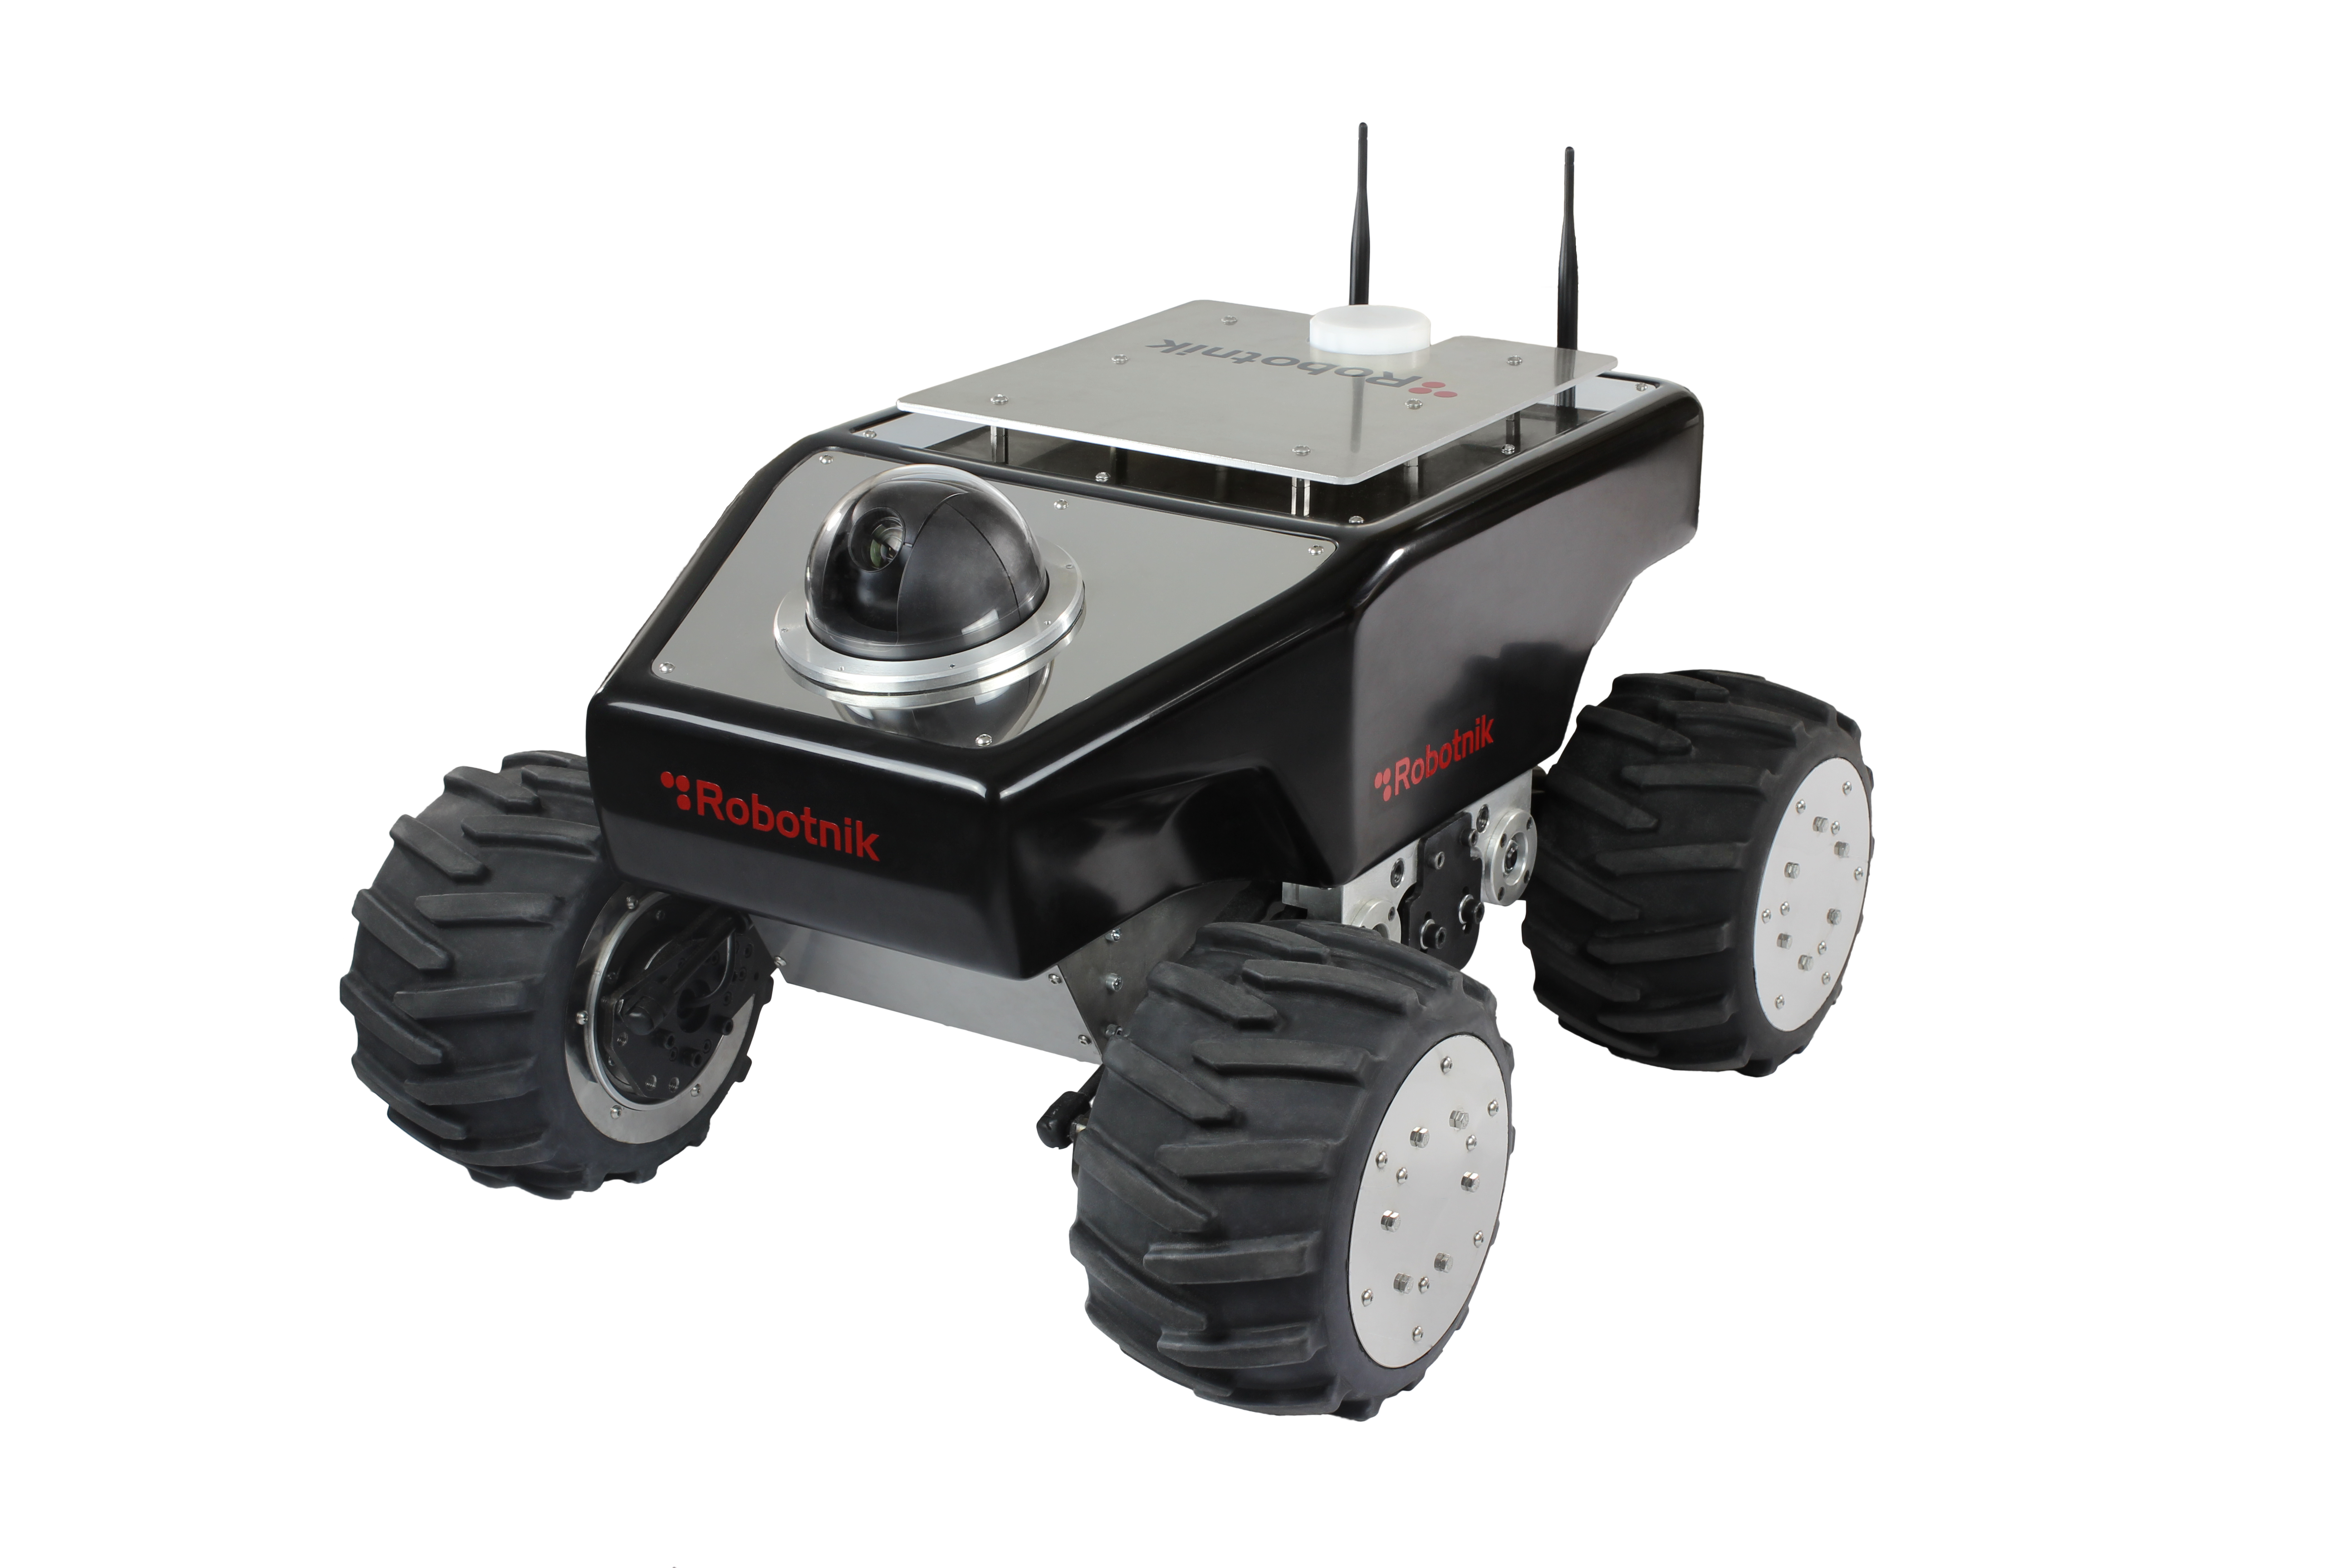
\includegraphics[width=\textwidth, height=\textwidth]{images/robot_movil.png}
    \caption{Robot móvil}
    \label{fig:f2}
  	\end{subfigure}
  	\begin{subfigure}[b]{0.25\textwidth}
    \includegraphics[width=1.3\textwidth, height=\textwidth]{images/robot_medico.png}
    \caption{Robot médico}
    \label{fig:f3}
  	\end{subfigure}
  	\begin{subfigure}[b]{0.25\textwidth}
    \includegraphics[width=0.7\textwidth, height=\textwidth]{images/robot_androide.png}
    \caption{Robot androide}
    \label{fig:f3}
  	\end{subfigure}
  	\caption{Tipos de robots en función de su utilidad.}
\end{figure}
	\end{itemize}


	\item En función de su operación:
	\begin{itemize}
		\item Robots teleoperados. Aquellos robots cuyas acciones que son controladas de manera remota por una persona. Este tipo de robots se utilizan principalmente en tareas que puedan suponer un riesgo de salud para las personas, pero que al mismo tiempo requieran un tratamiento humano para su elaboración (por ejemplo, robots para desactivación de bombas).
		
		\item Robots autónomos. Por el contrario, este tipo de robots son capaces de realizar tareas de manera independiente ya que son máquinas mucho más complejas y son dotadas con cierta inteligencia. Este tipo de robots son utilizados en algunos escenarios en los que el robot es capaz de analizar el entorno que le rodea para generar una respuesta por sí mismo. Este tipo de robots es el que utilizaremos para desarrollar este proyecto.
	\end{itemize}
\end{enumerate}

A día de hoy existen numerosas aplicaciones de la robótica en nuestra vida cotidiana, y cada vez son más los casos de uso debido a su gran utilidad y a la mejora que producen en la vida de las personas. El campo de la robótica está en continuo investigación y desarrollo, debido en gran parte a la gran velocidad con la que ha avanzado la tecnología en los últimos años. Algunos de los ejemplos más relevantes del uso de la robótica en nuestra vida cotidiana son; el coche autónomo de Tesla, dotado de cámaras y sensores que permiten que el coche sea capaz de circular de manera autónoma e identificar su entorno para actuar en consecuencia (detenerse en caso de que haya un peatón justo en frente, corregir la trayectoria en caso de pisar una línea continua…);  aspiradoras Roomba, capaces de identificar y memorizar la superficie aspirada para recorrer  y limpiar toda la vivienda de manera autónoma;  el robot DaVinci, un instrumento quirúrgico capaz de reproducir los movimientos de un cirujano sin latencia y con precisión, que permite reducir los temblores del cirujano y hace que pueda operar sentado de una manera más cómoda; centros logísticos de Amazon equipados con robots que ayudan a los humanos a seleccionar, clasificar, transportar y almacenar paquetes.
\\

Sin duda la robótica es un campo muy útil, en continuo desarrollo y de gran interés común, por lo que realizar un trabajo de fin de grado en este ámbito resulta interesante ya que es un tema que está a la orden del día y son muchos los casos de uso realizables en la vida real.


\section{Deep Learning en Visión Artificial}
Muchos de los robots actuales tienen una cámara como sensor principal que les permite tener cierto conocimiento del entorno en el que se encuentran, por lo que pueden actuar e interaccionar con los elementos que les rodean en consecuencia. Por tanto, estos robots se convierten en sistemas inteligentes cuya inteligencia está dotada principalmente por dos elementos: la cámara (visión artificial) y los algoritmos que procesan esas imágenes (Deep Learning).
\\

El \textit{Deep Learning} (aprendizaje profundo) es una rama de la ingeniería que permite a un ordenador crear conceptos y lógicas complejas a partir de otras más simples, todo ello mediante un aprendizaje automático. Los algoritmos de Deep Learning permiten crear un conocimiento en una máquina mediante un entrenamiento e intentan modelar abstracciones de alto nivel (por ejemplo, percepciones humanas tales como identificar distintos objetos en una imagen) utilizando arquitecturas compuestas de transformaciones no lineales múltiples. Una de las grandes ventajas del Deep Learning es que, a medida que aumenta la cantidad de datos y de ejemplos utilizados, mejora la precisión del algoritmo. \cite{Deep Learning}
\\

En un contexto más amplio, el \textit{Deep Learning} es una familia de técnicas dentro del Aprendizaje Automático, que es parte de la Inteligencia Artificial (IA). La IA que es la ciencia que estudia la inteligencia que es capaz de desarrollar una máquina mediante la programación. Dentro de la Inteligencia Artificial podemos encontrar el Aprendizaje Máquina (\textit{Machine Learning}), definido como la capacidad de las máquinas para aprender, construyendo modelos o patrones a partir de datos no procesados); el Aprendizaje de la Representación (\textit{Representation Learning}), que emplea el Aprendizaje Máquina para descubrir automáticamente representaciones o clasificaciones de datos sin procesar); y el Aprendizaje Profundo (\textit{Deep Learning}). En particular, el Deep Learning se caracteriza por ofrecer muy buenos resultados en detección de objetos en imágenes. El diagrama de Venn (Figura 1.2) muestra los subconjuntos de la Inteligencia Artificial. \cite{IA}
\\

Por otra parte, la Visión Artificial (\textit{Computer Vision}) es la rama de la ciencia que recopila todos los métodos para adquirir, procesar, analizar y comprender las imágenes del mundo real para que puedan ser procesadas por un ordenador. En concreto, en este proyecto combinaremos la visión artificial para obtener imágenes de un robot en un entorno real simulado y el \textit{Deep Learning}, para el procesamiento e interpretación de esas imágenes y así dotar de cierta inteligencia necesaria al robot para que sea capaz de actuar en función de las condiciones de su entorno. 

\renewcommand{\figurename}{Figura}		
\begin{figure}[h]
	\centering
	 \includegraphics[scale=0.5]{images/diagrama-venn.jpg}
	 \caption{Diagrama de Venn}
\end{figure}

\newpage
\subsection{Redes Neuronales Convolucionales (CNNs)}

Existen distintas técnicas para llevar a la práctica el \textit{Deep Learning}. Una de ellas son las Redes Neuronales Convolucionales (CNN). Las redes neuronales son modelos de aprendizaje automático que intentan emular las neuronas de los sistemas nerviosos biológicos. Al igual que un cerebro humano, las redes neuronales pretenden establecer conclusiones de los datos que obtienen. En concreto, las Redes Neuronales Convolucionales utilizan filtros convolucionales (múltiples filtros o capas por los que va pasando la información) para realizar esta función.
\\

La arquitectura de las Redes Neuronales Convolucionales se basa en utilizar distintos niveles o capas en los que después de cada uno de ellos se añade una función para realizar un mapeo causal no-lineal. Es decir, cada capa está formada por dos subcapas: una capa convolucional (que realiza una operación de convolución), y una capa de submuestreo (\textit{pooling}, que genera características a partir de cálculos estadísticos del resultado de la convolución). Todas estas capas están conectadas de  tal forma que a la salida de todas ellas se puedan obtener conclusiones a partir de los resultados obtenidos. Cuantas más capas posea una red neuronal, más probabilidad hay de que los resultados obtenidos sean acertados. En la Figura 1.3 podemos encontrar un ejemplo de una red neuronal convolucional que clasifica un número manuscrito al número digital que corresponde. \cite{Redes neuronales}

\renewcommand{\figurename}{Figura}		
\begin{figure}[h]
	\centering
	 \includegraphics[scale=0.45]{images/ejemplo_cnn.png}
	 \caption{Ejemplo de la arquitectura de una Red Neuronal Convolucional}
\end{figure}

Este trabajo se centra en la detección de objetos a través de imágenes, por lo que las Redes Neuronales Convolucionales son de gran utilidad ya que con ellas se puede procesar la imagen por secciones e identificar los objetos de manera más eficiente. Aplicando una red neuronal convolucional a nuestras imágenes podremos identificar el tamaño, la posición y el tipo de objeto que aparece en una imagen, siempre y cuando la clasificación del objeto identificado se encuentre dentro de las clases determinadas de la red neuronal. Para dicha implementación existen diversas plataformas tales como \texttt{Keras}, \texttt{TensorFlow}, \texttt{Caffe}, etc. En nuestro caso utilizaremos \texttt{TensorFLow} y, en concreto, TensorFlowjs, que es la librería para desarrollarlo en JavaScript. El motivo de esta elección es que utilizaremos nuestra red en un entorno web, por lo que el hecho de que exista dicha librería en lenguaje JavaScript nos facilitará la incorporación de la red a nuestro entorno. Además, TensorFlow dispone de numerosos modelos pre-entrenados que podremos usar sin la necesidad de entrenar previamente un modelo y etiquetar infinidad de imágenes.

Algunos ejemplos en la vida real de la aplicación de Deep Learning y redes neuronales en procesamiento de imágenes son; Google Photos y su algoritmo para reconocer rostros y organizar las imágenes de la galería; reconocimiento inteligente de defectos en las piezas de una fábrica a través de una cámara que va captando las piezas que pasan a través de una cinta; la creación de ImageNet, una base de datos de imágenes clasificadas cuya creación se ayudó de técnicas de Deep Learning para clasificar las imágenes; Autopilot, la función de conducción autónoma de los coches Tesla que utiliza algoritmos de Deep Learning para materializar las abstracciones de su entorno y poder identificar los objetos que rodean al coche en todo momento y lograr así una conducción autónoma. 

\section{Robótica en educación}

En virtud del auge que está sufriendo la robótica en los últimos años, cada vez son más los profesionales demandados en este campo. Debido a esto, en paralelo con el auge de la robótica, también ha aumentado de manera exponencial la enseñanza de la robótica en edades tempranas ya que aprender robótica puede ofrecernos una formación en diversos campos de forma simultánea: física, electrónica, informática...Además, el uso de aplicaciones de robótica refuerza la creatividad (a través del diseño de ideas y su desarrollo), el pensamiento crítico (pensamientos lógicos) y prepara a los niños para un futuro en el que la robótica adquirirá un papel fundamental en la sociedad. Poco a poco se han ido introduciendo materias de robótica en la enseñanza. Por ejemplo, en la Comunidad de Madrid y en muchas otras se ha incluido en los proyectos formativos asignaturas de robótica. En contexto universitario se han creado grados específicos de robótica, como el grado de robótica en la Universidad de Alicante o el Grado en ingeniería robótica en la Universidad  Rey Juan Carlos. Además, en estos últimos años se han desarrollado numerosas plataformas orientadas a este fin. Entre ellas podemos encontrar OpenRoberta, iRobot y Kibotics (que es la que usaremos para este proyecto). A continuación se detallan cada una de ellas.

\subsection{OpenRoberta}

Es una plataforma \footnote{https://lab.open-roberta.org/} \cite{Open Roberta} orientada a la programación por bloques en la que se pueden programar robots y otros sistemas hardware programables como \texttt{Arduino}, \texttt{BBC micro} y \texttt{Calliope mini}. El objetivo de OpenRoberta es simplificar los conceptos de programación para poder introducir esta materia en los colegios. Ofrece un entorno de programación basado en la nube y desarrollado en código abierto que permite su uso en cualquier navegador sin necesidad de instalación. Dispone de varios robots y sistemas (mBot, Arduino,etc) con múltiples motores y sensores que pueden ser configurados a través de bloques. Ofrece múltiples idiomas y no es necesario registrarse para utilizarlo.

\renewcommand{\figurename}{Figura}		
\begin{figure}[h]
	\centering
	 \includegraphics[scale=0.34]{images/openRoberta.jpg}
	 \caption{Interfaz de OpenRoberta}
\end{figure}

\newpage
\subsection{iRobot Education}

iRobot \cite{iRobot} es una empresa estadounidense que se dedica al diseño y fabricación de robots, principalmente orientados al uso en empresas, hogares e instituciones. Es conocida por el robot \textit{Roomba}, una aspiradora doméstica inteligente. Esta empresa ha creado iRobot Education \footnote{https://edu.irobot.com/}, una plataforma educativa destinada al aprendizaje de robótica. Esta empresa comercializa distintos robots, como por ejemplo el  robot móvil llamado \texttt{Create2}, muy parecido a su famoso aspirador Roomba, que los estudiantes y desarrolladores pueden programar para controlar los movimientos y el comportamiento del mismo de una manera sencilla a través de su plataforma. Otro robot que comercializan es el \texttt{iRobot Root rt0}, un robot con múltiples sensores (luz, movimiento...), con cámara, y con una superficie que permite introducir un lápiz de color para que el robot sea capaz de dibujar sobre una superficie en función del comportamiento programado. Esta plataforma es muy novedosa y  está destinado a aquellos estudiantes de secundaria y universidad, que empiezan a aprender robótica y a adquirir experiencia en programación, y sobre todo para familiarizarse tanto con el software como con el hardware.

\renewcommand{\figurename}{Figura}		
\begin{figure}[h]
\centering
  \begin{subfigure}[b]{0.24\textwidth}
  \centering
    \includegraphics[width=1.6\textwidth, height=\textwidth]{images/irobot.jpeg}
    \caption{Robot Create2}
    \label{fig:f1}
  \end{subfigure}\hspace{0.15\textwidth}
    \begin{subfigure}[b]{0.24\textwidth}
    \centering
    \includegraphics[width=1.6\textwidth, height=\textwidth]{images/irobot-r10.jpeg}
    \caption{Robot iRobot-r10}
    \label{fig:f2}
  	\end{subfigure}
  	\caption{Robots de iRobot Education}
\end{figure}

\newpage
\subsection{Kibotics} 

Es una plataforma \footnote{https://kibotics.org/} \cite{Kibotics} desarrollada por la Asociación de robótica e inteligencia artificial JdeRobot, destinada a la docencia \textit{STEM}. Este término hace referencia a \textit{Science, Technology, Engineering and  Mathematics} y se utiliza en términos de educación para apoyar la extensión del estudio de ingeniería, el inicio de la ingeniería, o en la escuela primaria. El objetivo de Kibotics es iniciar a niños y adolescentes en robótica y programación de robots. Se ejecuta en el navegador, por lo que no necesita instalación. Utiliza lenguajes intuitivos, como son Python y Scratch. Es especialmente interesante para los alumnos porque ofrece una gran variedad de robots programables tanto reales como simulados (PiBot, drones, Fórmula 1), y permite el desarrollo de prácticas avanzadas de visión artificial (robots con cámara). Esta es la plataforma que se va a utilizar para desarrollar este trabajo.

\renewcommand{\figurename}{Figura}
\begin{figure}[h]
\centering
	\begin{subfigure}[h]{\textwidth}
	\centering
	 \includegraphics[scale=0.15]{images/scratch+websim.png}
	 \caption{Scratch en Kibotics}
	\end{subfigure}
	\begin{subfigure}[h]{\textwidth}
	\centering
	 \includegraphics[scale=0.15]{images/python+websim.png}
	 \caption{Python en Kibotics}
	\end{subfigure}
	\caption{Interfaz de Kibotics con distintos lenguajes de programación}
\end{figure}

\chapter{Objetivos}
Una vez puesto en contexto el marco en el que se engloba este trabajo, en este capítulo se definen los objetivos generales y específicos planteados para su realización. A continuación se presentan los requisitos adicionales necesarios que deseamos cumplan las soluciones alcanzadas. Finalmente se define la metodología llevada a cabo para la consecución de los objetivos.

\section{Objetivos}
El objetivo general de este trabajo es aumentar la funcionalidad de visión artificial de los robots de la plataforma Kibotics y que sea fácil de utilizar por niños. Actualmente los robots de dicha plataforma cuentan con una serie de funciones de visión que les permiten cierta interacción con su entorno. Por ejemplo, las funciones disponibles son: \texttt{getImage()}, que devuelve una imagen capturada por la cámara del robot o \texttt{getObjectColorRGB(lowval, highval)} que devuelve el centro y el área de un objeto de un determinado color detectado en una imagen. 
\\

Estas funciones son muy útiles pero pueden llegar a ser poco intuitivas para un usuario principiante en el ámbito de la programación. Además no permiten la percepción de objetos más realistas y complejos. Es por ello el objetivo de este trabajo es crear nuevas funciones que sean potentes y sencillas de usar para incorporarlas en el API de los robots de Kibotics. En concreto, los subobjetivos específicos de este trabajo se plantean en tres puntos:

\begin{enumerate}
\item Ampliar el API de los robots de Kibotics con una función que permita detectar la carretera desde la visión subjetiva del robot. Resultará útil para ejercicios atractivos de un robot en una ciudad simulada. En concreto dicha función será \texttt{dameCentroCarretera()} que utilizará OpenCVjs como herramienta para su desarrollo.


\item Ampliar el API de los robots de Kibotics con una función que permita detectar en la imagen de los robots distintos objetos de interés como semáforos, personas, señales de tráfico, etc. Esta nueva función pretende materializar las redes neuronales y la técnica de Deep Learning. En concreto dicha función será \texttt{ dameObjetoCiudad()} que utilizará TensorFlowjs como herramienta para detectar objetos en las imágenes que capta el robot.

\item Validación experimental desarrollando dos comportamientos robóticos que utilicen sendas funciones y saquen partido de esa funcionalidad. Para ello, se pretende crear un nuevo entorno en el que situar uno de los robots de Kibotics y desarrollar los objetivos específicos mencionados anteriormente. En concreto se creará un entorno simulado que imite una pequeña ciudad con distintos elementos y que el robot utilizado represente un coche que circula por la ciudad.
\end{enumerate}

\subsection{Requisitos}
El desarrollo de este proyecto está condicionado por el cumplimiento de una serie de requisitos:

\begin{itemize}
\item La plataforma para el desarrollo de este trabajo será Kibotics.
\item El lenguaje de programación empleado para crear las nuevas funciones del API de los robots de Kibotics será JavaScript.
\item Las nuevas funciones creadas para el API de los robots de Kibotics tendrán que ser sencillas de usar, ya que están destinadas a que las usen niños y adolescentes que están empezando a programar. Además sus detecciones tienen que ser robustas, es decir, que tengan un correcto funcionamiento y permitan basar comportamientos robóticos en ellas.
\end{itemize}

\section{Metodología}
Para lograr los objetivos mencionados anteriormente, se han utilizado distintas herramientas y mecanismos que han permitido un desarrollo óptimo del trabajo y un control y seguimiento del mismo. 
\\

En primer lugar, se han establecido reuniones semanales con los tutores de este trabajo en las que se realizaban la planificación de tareas, correcciones de las tareas ya realizadas y establecimiento de objetivos para la siguiente semana. Además se ha utilizado un canal de Slack \footnote{http://jderobot.slack.com/} que ha permitido una comunicación constante para la resolución de dudas e inquietudes. En este canal de Slack se disponía además de un canal compartido con todos los miembros integrantes y desarrolladores de la plataforma Kibotics en el que se han compartido ideas y se han resuelto dudas. También se ha utilizado el correo electrónico para el intercambio de información, documentos y mensajes.
\\

En segundo lugar, se ha creado una bitácora y un repositorio de GitHub \footnote{https://github.com/RoboticsLabURJC/2019-tfg-jorge-cruz} para ir reflejando los progresos semanales y para dejar constancia de los objetivos que se iban cumpliendo. En dicho repositorio semanalmente se han escrito los progresos realizados durante la semana. Este repositorio también ha servido como referencia para llevar un control y un seguimiento del proyecto. Como plataforma complementaria se ha utilizado Youtube y se ha creado un canal \footnote{https://www.youtube.com/channel/UCe2zYaXRPMc1qCQWzTVKvgQ} para la compartición de vídeos y para mostrar al resto del equipo los progresos que se iban consiguiendo.

\chapter{Infraestructura}
En este capítulo se describen las diferentes herramientas software utilizadas en el desarrollo de este TFG. Especialmente se detalla la plataforma educativa Kibotics en la se encuadran todos los desarrollos, así como las bibliotecas de procesamiento de imágenes.

\section{Lenguaje JavaScript}
JavaScript \footnote{https://developer.mozilla.org/es/docs/Web/JavaScript} \cite{JavaScript} es un lenguaje de programación interpretado,  de alto nivel, orientado a objetos, débilmente tipado (permite flexibilidad en el manejo de variables) y que se apoya en otros lenguajes como Java o C. Es el lenguaje más utilizado para desarrollo web, ya que los navegadores tienen la capacidad de interpretar el código JavaScript integrado en las páginas web. Este código se integra dentro de los ficheros HTML (aquellos que se encargan de gestionar todo lo que se muestra en pantalla) para realizar operaciones y definir la lógica de la página en el lado del cliente, ya que tiene acceso al DOM \footnote{https://developer.mozilla.org/es/docs/DOM} (Document Object Model),  permite la modificación de etiquetas HTML, envío de mensajes al navegador (alertas) y generación de gráficos en canvas\footnote{https://developer.mozilla.org/es/docs/Web/HTML/Canvas} entre  muchas otras funciones. Existen numerosas API's en JavaScript del lado del cliente que no son parte del lenguaje pero que permiten utilizar numerosas funcionalidades y abstraer problemas complejos. Un ejemplo de ello es el API de Geolocalización, que permite obtener datos de ubicación a través de métodos de alto nivel (como por ejemplo \texttt{getCurrentPosition}). Esto permite que el programador no se tenga que preocupar por usar un código complejo de bajo nivel para comunicarse con el hardware GPS del dispositivo. 
\\

Para este proyecto se ha utilizado JavaScript para programar la inteligencia de la aplicación web que corre en el navegador y, en concreto, el comportamiento del robot PiBot para que este sea capaz de circular de forma autónoma por una carretera en un entorno simulado, identificando los elementos de su entorno como señales de tráfico, semáforos o personas. Para conseguir esta funcionalidad se ha hecho uso de dos bibliotecas de JavaScript, OpenCVjs y TensorFlowjs, descritas a continuación.

\section{Kibotics}
Kibotics \cite{Kibotics} es una plataforma desarrollada por la Asociación de robótica e inteligencia artificial \\JdeRobot, destinada a la educación en robótica. En esta plataforma se pueden encontrar diversos ejercicios en los que el estudiante puede programar el comportamiento de un robot en diferentes situaciones: un coche de fórmula1 que sigue una línea en un circuito de carreras, un robot aspirador que se mueve por una habitación, un robot móvil que sigue una pelota, etc.Para programar estos comportamientos el usuario puede elegir entre dos lenguajes: Python o Scratch. Por debajo de estos dos lenguajes, toda la lógica del entorno web está programada en JavaScript.
\\

La plataforma ha sido presentada en el primer capítulo. Profundizando un poco más en su estructura interna, Kibotics sigue para cada robot el modelo cuerpo + cerebro. El cuerpo lo materializa el simulador Websim, basado en A-Frame, y el cerebro lo programa el usuario utilizando lenguaje Python o Scratch, que se traducen a JavaScript. El programador tiene a su disposición varias funciones para acceder a los sensores y actuadores del robot. Estas funciones se agrupan en el robotAPI. Típicamente el programa que ejecuta el cerebro accede continuamente a los sensores (usando robotAPI) y decide qué hacer en cada momento y qué ordenar a los motores del robot. El robotAPI está compuesto de cuatro partes; \textit{HalRobotAPI}: contiene todas las funciones relacionadas con los movimientos del robot tales como avanzar, parar, establecer un ángulo de giro, etc; \textit{consoleRobotAPI}: funciones que permiten al usuario comunicarse con la consola del navegador; \textit{utilsRobotAPI}: funciones auxiliares como por ejemplo la función \textit{sleep}, que permite congelar el robot durante unos segundos; \textit{visionRobotAPI}: contiene todas las funciones de visión artificial que pueden utilizar los robots tales como obtener una imagen de la cámara del robot, filtrar el color en una imagen, etc. Esta última parte es en la que se centra el trabajo, enfocado a incrementar nuevas funcionalidades de la misma.
\\

El funcionamiento interno de Kibotics está basado en un diseño formado por dos planos de actuación: un primer plano, formado por los robots, sus sensores, actuadores, y el robotAPI; y un segundo plano formado, por un web worker en el que se incluye el código del usuario que programa el comportamiento del robot, y un robotAPI de segundo plano que también permite ordenar acciones al robot. La conexión entre el primer y el segundo plano se hace a través de un miniproxy que se encarga de enviar mensajes en ambos sentidos para el intercambio de información (instrucciones o parámetros de los sensores del robot). El motivo de este diseño es conseguir una división de tareas en dos planos de actuación, para realizar aquellas necesarias en un primer plano (acceso nativo a los sensores y actuadores del robot) y aquellas que puedan permitir una demora (procesamiento de las imágenes del robot, interpretación de los sensores como infrarrojos…) realizarlas en un segundo plano, para que no bloqueen el flujo de ejecución del programa. En un primer prototipo, las nuevas funcionalidades del robotAPI  (Aplication Programming Interface) de los robots se han programado en el API de primer plano, para comprobar su eficiencia y utilidad y en futuro programarlas en el robotAPI de segundo plano.


\renewcommand{\figurename}{Figura}		
\begin{figure}[p]
	\centering
	 \includegraphics[scale=0.4]{images/kibotics.png}
	 \caption{Flujo de datos de Kibotics entre el código de usuario y los sensores del robot.}
\end{figure}

\newpage
\section{A-Frame}
A-Frame \footnote{https://aframe.io/} \cite{A-Frame} es una plataforma de código abierto destinada a crear y simular experiencias 3D, de realidad virtual y de realidad aumentada en la web. Se caracteriza por la gran facilidad de crear escenarios tridimensionales, simular entornos de la vida real y la facilidad que ofrece para añadir modelos sofisticados en diferentes formatos. Estas escenas son fácilmente configurables y modificables a través de ficheros, por lo que cambiar las luces de  una escena, los controles, los tamaños de los objetos, etc, es tan sencillo como cambiar una línea de código. Por ello A-Frame ofrece una gran versatilidad y utilidad, ya que toda una escena puede ser configurada en un archivo JavaScript e incluirse en un fichero HTML para su visualización web. Además, A-Frame es compatible con la mayoría de las bibliotecas (React, AngularJS, D3.js, Vue.js) y navegadores web existentes (Firefox, Google Chrome, Opera). 
\\

Algunos de los usos más comunes de A-Frame son el desarrollo de videojuegos, la recreación de entornos reales para realizar simulaciones y la  recreación de experiencias 3D ya que A-Frame tiene compatibilidad con Vive, Rift, Windows Mixed Reality, Daydream, GearVR y CardBoard por lo que se puede crear una escena en A-Frame y posteriormente ser usada en un entorno de simulación para, por ejemplo, verse inmerso en ella utilizando gafas de realidad virtual. A-Frame es el motor de simulación que se utiliza en la plataforma Kibotics y que permite al usuario visualizar la escena sobre la que se programa el comportamiento de un robot.
\\

Esta es la plataforma que usaremos en este proyecto para simular nuestro entorno; una mini-ciudad recreada con una alfombra infantil con carreteras, un robot móvil, y diferentes elementos de la ciudad, tales como señales de tráfico, peatones y semáforos que van cambiando de color. La versión de A-Frame utilizada en este trabajo ha sido la versión 1.0.4

\renewcommand{\figurename}{Figura}		
\begin{figure}[h]
	\centering
	 \includegraphics[scale=0.17]{images/a-frame.png}
	 \caption{Ejemplo de un mundo 3D virtual con A-Frame}
\end{figure}

\section{Blender}
Blender \footnote{https://www.blender.org/} \cite{Blender} es una herramienta de código abierto destinada al diseño y animación 3D. A través de una interfaz gráfica se pueden crear objetos, personajes, escenas, animaciones y todo tipo de diseño tridimensional. Blender ofrece diversas características tales como el modelado (creación de objetos en un espacio tridimensional de manera digital), tracking (especificación del comportamiento y características de un objeto), animación (mediante secuencia de fotogramas) e iluminación (ajustar la luz deseada a la escena para cada objeto en cuanto a intensidad, color o posición). Es compatible con todas las versiones de Windows, macOS, GNU/Linux, Solaris, FreeBSD e IRIX.
\\

Para insertar los objetos creados en Blender en un entorno de A-Frame se deben exportar dichos objetos en formato GL Transmssion Format (glTF) ya que este formato minimiza el tamaño de los ficheros permitiendo así ver con fluidez las animaciones creadas. A nivel profesional, podemos encontrar diversos ejemplos del uso de Blender , como la pre-visualización de escenas para películas como \textit{Spider-Man} o \textit{Capitán América }o la realización de largometrajes (\textit{Plumíferos} \footnote{https://es.wikipedia.org/wiki/Plumíferos}) y cortometrajes (\textit{Elephant Dream} \footnote{https://orange.blender.org/}).
\\

En este proyecto se ha utilizado Blender para el diseño de los objetos que conforman la ciudad simulada en el nuevo escenario robótico 3D: señales de tráfico (señal de stop), semáforo animado que cambia de color y peatones animados que simulan la acción de caminar. La versión de Blender utilizada en este trabajo ha sido la versión 2.90.1.

\renewcommand{\figurename}{Figura}		
\begin{figure}[h]
	\centering
	 \includegraphics[scale=1]{images/blender.jpg}
	 \caption{Interfaz gráfica de Blender}
\end{figure}

\section{OpenCVjs}
OpenCVjs \footnote{http://opencv.org} \cite{OpenCVjs} (Open Source Computer Vision Library) es una biblioteca de código abierto destinada a usarse en código JavaScript que incluye diversos algoritmos de visión artificial. Tiene una estructura modular; los algoritmos están organizados en bibliotecas estáticas, entre los que podemos encontrar: \textit{core funcionality, image processing, video analysis…} Esta librería resulta especialmente interesante en el campo de la visión artificial, ya que ofrece una funcionalidad para el robot con imágenes muy compleja pero a la vez muy intuitiva y cercana a las \textit{funciones del sistema humano}, como por ejemplo identificar un color, situar en una imagen un determinado color, detectar líneas y círculos, entre muchas otras. Además, ofrece  otras muchas funciones más propias del tratamiento de imágenes, como detectar bordes, rotar o recortar imágenes, modificar el espacio de color, filtrar un color en la imagen, erosionar o suavizar los bordes de una imagen, etc.
\\

En este proyecto se ha utilizado la biblioteca de OpenCVjs para realizar filtros de color en las imágenes que capta el robot PiBot, ya que dichos filtros son una de las herramientas que ofrece la biblioteca OpenCVjs. Estos filtros de color sobre la imagen que capta el robot se realizan con el fin de separar el color de la carretera respecto al entorno circundante. La versión de OpenCVjs utilizada en este trabajo ha sido la versión 3.3.1.

\begin{figure}[h]
\begin{subfigure}{.5\textwidth}
  \centering
  \includegraphics[width=.7\linewidth]{images/imagen.JPG}  
  \caption{Imagen original}
  \label{fig:sub-first}
\end{subfigure}
\begin{subfigure}{.5\textwidth}
  \centering
  \includegraphics[width=.7\linewidth]{images/gris.JPG}  
  \caption{Blanco y negro}
  \label{fig:sub-second}
\end{subfigure}


\begin{subfigure}{.5\textwidth}
  \centering
  \includegraphics[width=.7\linewidth]{images/blur.JPG}  
  \caption{Filtro gaussiano}
  \label{fig:sub-third}
\end{subfigure}
\begin{subfigure}{.5\textwidth}
  \centering
  \includegraphics[width=.7\linewidth]{images/bordes.JPG}  
  \caption{Detección de bordes}
  \label{fig:sub-fourth}
\end{subfigure}
\caption{Ejemplos de procesamiento de imágenes con OpenCVjs}
\label{fig:fig}
\end{figure}

\newpage
\section{TensorFlowjs}
TensorFlowjs \footnote{https://www.tensorflow.org/} \cite{TFjs} es una biblioteca de código abierto destina a realizar una computación numérica de alto rendimiento de una forma eficiente en la web. Está desarrollado por Google Brain Team y ofrece numerosas herramientas para realizar tareas de aprendizaje automático (Machine Learning). Con esta biblioteca se pueden construir y entrenar redes neuronales para posteriormente usarlas en clasificación y detección de objetos, patrones, correlaciones, o razonamientos similares a los de un cerebro humano. Además de construir y entrenar modelos, también se pueden ejecutar modelos existentes.
\\

TensorFlowjs es una parte de la herramienta TensorFlow en sí misma, que incluye esta biblioteca JavaScript para que pueda ejecutarse, por ejemplo, dentro de páginas web. Está diseñado para realizar operaciones en segundo plano, lo que hace que la utilización de sus funciones no bloquee el flujo de ejecución del hilo principal y puedan seguir realizando operaciones de manera muy rápida en comparación con otras bibliotecas matemáticas de alto nivel (como por ejemplo NumPy). Además, está optimizado para un uso paralelo del hardware de la GPU, lo que hace que aumente el rendimiento al reducir el tiempo entre inferencias. Hoy en día, esta biblioteca de código abierto se utiliza en ámbitos de investigación y en algunos productos de Google, como por ejemplo el reconocimiento de voz, el traductor que permite traducir textos en imágenes en tiempo real, o el reconocimiento de imágenes de la galería de Google Photos.
\\

En este proyecto se ha utilizado TensorFlowjs para hacer uso de los modelos de redes neuronales pre-entrenados e integrarlos dentro de la plataforma Kibotics para que los robots de la misma puedan realizar operaciones neuronales. Estas operaciones neuronales permitirán a los robots identificar distintos elementos en las imágenes captadas por las cámaras que incorporan. La versión de TensorFlowjs utilizada en este trabajo ha sido la versión 1.0.0.

\chapter{Robot Autónomo en Ciudad Simulada}

En este capítulo se describe el proceso llevado a cabo para dotar al robot PiBot equipado con una cámara de la inteligencia necesaria para ser capaz de circular por una carretera en una ciudad simulada siguiendo el trazo de la misma e interactuando con los obstáculos que se encuentre (semáforos, personas y señales de stop). En primer lugar se presenta el robot utilizado para el desarrollo de este trabajo. En segundo lugar se explica el entorno simulado para su desarrollo. Finalmente se describen dos tipos de comportamientos programados; \textit{\textbf{sigue carretera básico}}: el robot sigue el curso de la carretera; \textit{\textbf{sigue carretera avanzado}}: además de seguir la trayectoria de la carretera el robot es capaz de actuar en función de los obstáculos que se encuentre. 

\section{Robot PiBot}
El robot utilizado para realizar este Trabajo Fin de Grado ha sido el robot PiBot, uno de los robots disponibles en la plataforma Kibotics para poder programar su comportamiento. Este robot se caracteriza por ser un robot móvil y por disponer de un hardware que le permite realizar cierta interacción con su entorno. En concreto, el robot PiBot está dotado con sensores infrarrojos y sensores infrasonidos para la detección de objetos próximos a él, y de una cámara frontal que le permite captar imágenes de su entorno a medida que el robot se mueve. El nombre PiBot hace referencia a que todos los sensores y actuadores del robot en su versión física están conectados a una Raspberry Pi para el control de los mismos (Pi-Bot). El motivo de la elección de este robot para realizar este trabajo es que gracias a la cámara que dispone se pueden realizar todas las tareas de visión artificial a través de las imágenes que capta. Estas imágenes serán procesadas, analizadas y permitirán materializar el comportamiento del robot en función de las mismas.

\renewcommand{\figurename}{Figura}		
\begin{figure}[!h]
\centering
  \begin{subfigure}[b]{0.49\textwidth}
  \centering
    \includegraphics[width=0.7\textwidth, height=0.5\textwidth]{images/cap4/pibot-frontal.png}
    \label{fig:f1}
  \end{subfigure}
  \hfill
  \begin{subfigure}[b]{0.49\textwidth}
  \centering
    \includegraphics[width=0.7\textwidth, height=0.5\textwidth]{images/cap4/pibot-lateral.png}
    \label{fig:f2}
  \end{subfigure}
  \caption{Robot PiBot simulado}
\end{figure}

\newpage
\section{Ciudad Simulada}

Se ha recreado un entorno con el objetivo de introducir el robot PiBot dentro y que sea capaz de  moverse y actuar en él. El propósito de este entorno es simular una ciudad interactiva pero conservando una estética infantil y educativa. Es por eso que la ciudad no es fotorealista y se ha buscado una apariencia más simple y vistosa, parecida a la de dibujos animados. Este entorno está compuesto por un conjunto de modelos y configuraciones (posición, tamaño, iluminación...) agrupados en un un fichero \textbf{.json}. Este tipo de ficheros son entendibles por el entorno de realidad virtual A-Frame en el que está basado el simulador de Kibotics.

\subsection{Alfombra Infantil}
Se disponía de una alfombra real de dimensiones 2mx3m que ha sido digitalizada para usarse como base de la ciudad simulada en Kibotics, y en particular en el simulador basado en A-Frame. Esta base imita las carreteras de una ciudad con intersecciones, rotondas y líneas curvas. Se ha considerado que es un entorno interesante ya que plantea distintos puntos en los que el robot tendrá que tomar decisiones, no es simplemente una carretera de un carril en línea recta.

\renewcommand{\figurename}{Figura}		
\begin{figure}[!h]
\centering
  \begin{subfigure}[b]{0.49\textwidth}
  \centering
    \includegraphics[width=0.9\textwidth, height=0.7\textwidth]{images/cap4/alfombra-real.jpeg}
    \label{fig:f1}
    \caption{Alfombra real}
  \end{subfigure}
  \hfill
  \begin{subfigure}[b]{0.49\textwidth}
  \centering
    \includegraphics[width=0.9\textwidth, height=0.7\textwidth]{images/cap4/alfombra.jpg}
    \label{fig:f2}
    \caption{Alfombra digitalizada}
  \end{subfigure}
  \caption{Alfombra infantil}
\end{figure}


\newpage
\subsection{Señal de Stop}
Se ha modelado una señal de Stop en Blender a partir de las figuras primitivas geométricas básicas que ofrece dicho software (cubos, cilindros, conos...). Para insertar este modelo en el mundo basta con añadir el siguiente código al fichero de configuración del mismo, que será interpretado por A-Frame:

\begin{lstlisting}[backgroundcolor = \color{light-gray},
				   aboveskip = 2em,
				   belowskip = 2em,
                   xleftmargin = 2cm,
                   framexleftmargin = 1em,
                   basicstyle=\small]
{
 "tag": "a-gltf-model",
 "attr": {
	"position": { "x":-7, "y":-0.1, "z":11},
	"scale": { "x":-0.2, "y":0.2, "z":0.2},
	"rotation": {"x":0, "y":0},
	"src": "../assets/models/alfombra/StopSign.glb",
	"animation-mixer": "loop: repeat"
	}
}
\end{lstlisting}

\renewcommand{\figurename}{Figura}		
\begin{figure}[h]
	\centering
	 \includegraphics[scale=0.35]{images/cap4/stop.png}
	 \caption{Señal de Stop}
\end{figure}



\subsection{Semáforo animado}
Se ha modelado también una señal de tráfico en Blender a partir de las figuras primitivas geométricas básicas que ofrece dicho software (cubos, cilindros, conos...). Además, se han añadido animaciones para que el color del semáforo vaya cambiando cada cierto intervalo de tiempo. Esto permitirá mayor interacción del robot PiBot con dicho elemento, ya que además de identificar que hay un semáforo, tendrá que identificar el color para actuar en consecuencia. Para insertar este modelo en el mundo simulado basta con añadir el siguiente código al fichero de configuración del mismo, que será interpretado por A-Frame:

\newpage
\begin{lstlisting}[backgroundcolor = \color{light-gray},
				   aboveskip = 2em,
				   belowskip = 2em,
                   xleftmargin = 2cm,
                   framexleftmargin = 1em,
                   basicstyle=\small]
{
 "tag": "a-gltf-model",
 "attr": {
	"position": { "x":-3.28, "y":-0.1, "z":0.60},
	"scale": { "x":-0.12, "y":0.12, "z":0.12},
	"rotation": {"x":0, "y":70},
	"src": "../assets/models/alfombra/semaforo_animado.glb",
	"animation-mixer": "loop: repeat"
	}
}
\end{lstlisting}

\renewcommand{\figurename}{Figura}		
\begin{figure}[h]
  \begin{subfigure}[b]{0.3\textwidth}
    \includegraphics[width=\textwidth, height=1.2\textwidth]{images/cap4/rojo.png}
    \label{fig:f1}
  \end{subfigure}
  \hfill
  \begin{subfigure}[b]{0.3\textwidth}
    \includegraphics[width=\textwidth, height=1.2\textwidth]{images/cap4/amarillo.png}
    \label{fig:f2}
  \end{subfigure}
  \hfill
    \begin{subfigure}[b]{0.3\textwidth}
    \includegraphics[width=\textwidth, height=1.2\textwidth]{images/cap4/verde.png}
    \label{fig:f2}
  \end{subfigure}
  \caption{Semáforo simulado}
\end{figure}



\subsection{Peatones animados}
En la plataforma de Kibotics ya se disponía de modelos animados que simulaban peatones andando. Se han incorporado al fichero de la ciudad simulada mediante el siguiente código:

\begin{lstlisting}[backgroundcolor = \color{light-gray},
				   aboveskip = 2em,
				   belowskip = 2em,
                   xleftmargin = 2cm,
                   framexleftmargin = 1em,
                   basicstyle=\small]
{
 "tag": "a-gltf-model",
 "attr": {
	"position": { "x":-3.28, "y":-0.1, "z":6},
	"scale": { "x":1, "y":1, "z":1},
	"rotation": {"x":0, "y":-90},
	"src": "../assets/models/alfombra/person2.glb",
	"animation-mixer": "loop: repeat",
	"animation": "property: position; from: -1.28 -0.1 6 ;
	to: -13.28 -0.1 6; dur: 40000; loop: true"
 }
}
\end{lstlisting} 

A través de este código se puede configurar la posición inicial y final del movimiento de un peatón. De este modo se situarán distintos peatones repartidos por distintos puntos en la ciudad simulada, pudiendo configurar algunos de ellos para que estén continuamente cruzando pasos de cebra. Esto implicará una mayor interacción con el robot PiBot ya que habrá mayor probabilidad de que los peatones aparezcan en el radio de visión del robot a lo largo de su trayectoria.
\hfill \break

\renewcommand{\figurename}{Figura}		
\begin{figure}[!h]
\centering
  \begin{subfigure}[b]{0.49\textwidth}
  \centering
    \includegraphics[width=0.3\textwidth, height=0.5\textwidth]{images/cap4/person.jpg}
    \label{fig:f1}
  \end{subfigure}
  \hfill
  \begin{subfigure}[b]{0.49\textwidth}
  \centering
    \includegraphics[width=0.3\textwidth, height=0.5\textwidth]{images/cap4/person2.jpg}
    \label{fig:f2}
  \end{subfigure}
  \caption{Peatones animados}
\end{figure}

\hfill \break
\hfill \break

Además, al fichero de configuración del mundo se ha añadido un cielo azul para completar toda la escena. En la Figura 4.6 se muestran todos los elementos mencionados anteriormente integrados en la ciudad simulada.
\hfill \break
\hfill \break
\hfill \break
\renewcommand{\figurename}{Figura}		
\begin{figure}[h]
	\centering
	 \includegraphics[scale=0.35]{images/cap4/ciudad-simulada.png}
	 \caption{Elementos de la ciudad simulada}
\end{figure}

\newpage
\section{Aplicación robótica Sigue-Carretera Básico}
En este primer ejercicio se pretende dotar al robot PiBot de la inteligencia necesaria para que sea capaz de circular de manera autónoma por una carretera siguiendo el trazo de la misma, sin desviarse y a una velocidad constante (sin parones ni aceleraciones descompensadas). Para ello, este comportamiento se divide en dos partes que se ejecutan en iteraciones continuamente, en un bucle de control típico de comportamientos robóticos reactivos; \textbf{percepción}: el proceso mediante el cual el robot capta una imagen y es capaz de identificar la posición en la que se encuentra respecto a la carretera; \textbf{actuación}: en función de la posición en la que se encuentre, el robot se moverá de una manera o de otra.


\subsection{Percepción visual}

Para identificar la posición en la que se encuentra el robot PiBot respecto a la carretera primero hay que identificar la carretera en la imagen. Para ello se ha utilizado OpenCVjs como herramienta para utilizar filtros de color y poder transformar la imagen de la cámara del robot en una imagen binaria en la que los píxeles blancos representen la carretera y los píxeles negros el resto de información de la imagen que no interesa. A continuación se describe el proceso realizado:
\\

1.- Captura de la imagen de la cámara del robot PiBot utilizando el interfaz de programación robotAPI que la plataforma Kibotics ofrece para que los usuarios programen sus aplicaciones robóticas.

\begin{lstlisting}[backgroundcolor = \color{light-gray},
				   aboveskip = 1em,
				   belowskip = 2em,
                   xleftmargin = 2cm,
                   framexleftmargin = 1em,
                   basicstyle=\small]
var imagen = myRobot.dameImagen();
\end{lstlisting}

2.- Filtrar el color gris en la imagen capturada, que es el color del asfalto de la carretera en las imágenes de la cámara del robot PiBot.

\begin{lstlisting}[backgroundcolor = \color{light-gray},
				   aboveskip = 1em,
				   belowskip = 2em,
                   xleftmargin = 2cm,
                   framexleftmargin = 1em,
                   basicstyle=\small]
let lower = [50, 40, 40, 0];
let higher = [100, 90, 255, 255];
let src = cv.imread(imagen);
let dst = new cv.Mat();
let low = new cv.Mat(src.rows, src.cols, src.type(), lower);
let high = new cv.Mat(src.rows, src.cols, src.type(), higher);
cv.inRange(src, low, high, dst);
\end{lstlisting}

3.- Realizar transformaciones morfológicas: erosión y dilatación. Este paso se realiza para evitar falsos positivos. Es decir, evitar que pequeños puntos de la imagen que tienen el mismo color que la carretera sean identificados como parte de la carretera.

\begin{lstlisting}[backgroundcolor = \color{light-gray},
				   aboveskip = 1em,
				   belowskip = 2em,
                   xleftmargin = 2cm,
                   framexleftmargin = 1em,
                   basicstyle=\small]
let M = cv.Mat.ones(5, 5, cv.CV_8U);
let anchor = new cv.Point(-1, -1);
cv.dilate(dst, dst, M, anchor, 1, cv.BORDER_CONSTANT,
		 cv.morphologyDefaultBorderValue());
cv.erode(dst, dst, M, anchor, 3, cv.BORDER_CONSTANT,
		 cv.morphologyDefaultBorderValue());
\end{lstlisting}

4.- Finalmente se aplica un suavizado a la imagen para eliminar el ruido de la misma.

\begin{lstlisting}[backgroundcolor = \color{light-gray},
				   aboveskip = 2em,
				   belowskip = 2em,
                   xleftmargin = 2cm,
                   framexleftmargin = 1em,
                   basicstyle=\small]
cv.medianBlur(dst, dst, 5);
\end{lstlisting}

\begin{figure}[h]
\begin{subfigure}{.5\textwidth}
  \centering
  \includegraphics[width=.7\linewidth, height=.65\linewidth]{images/cap4/camara-pibot.png}  
  \caption{Imagen desde la cámara del PiBot}
  \label{fig:sub-first}
\end{subfigure}
\begin{subfigure}{.5\textwidth}
  \centering
  \includegraphics[width=.7\linewidth]{images/cap4/filtro-color.png}  
  \caption{Filtro de color}
  \label{fig:sub-second}
\end{subfigure}
\begin{subfigure}{.5\textwidth}
  \centering
  \includegraphics[width=.7\linewidth]{images/cap4/erosion-dilatacion.png}  
  \caption{Erosión y dilatación}
  \label{fig:sub-third}
\end{subfigure}
\begin{subfigure}{.5\textwidth}
  \centering
  \includegraphics[width=.7\linewidth]{images/cap4/erode.png}  
  \caption{Suavizado}
  \label{fig:sub-fourth}
\end{subfigure}
\caption{Proceso de filtrado del color de la carretera de una imagen del robot PiBot}
\label{fig:fig}
\end{figure}

Llegados a este punto, se dispone de una imagen binaria en la que los píxeles blancos representan la carretera y los píxeles negros el resto de información que se pretende evitar. Finalmente, para calcular el centro de la carretera, se aplica la función de OpenCVjs \textit{cv.moments} que nos aproxima el centro de un rectángulo que encierra todos los píxeles blancos de la imagen. De este modo se obtiene de una forma bastante aproximada el centro de la carretera.

\newpage
\begin{lstlisting}[backgroundcolor = \color{light-gray},
				   aboveskip = 2em,
				   belowskip = 2em,
                   xleftmargin = 2cm,
                   framexleftmargin = 1em,
                   basicstyle=\small]
let src2 = dst;
let dst2 = cv.Mat.zeros(src2.rows, src2.cols, cv.CV_8UC3);
let contours = new cv.MatVector();
let hierarchy = new cv.Mat();
cv.findContours(src2, contours, hierarchy, cv.RETR_CCOMP,
				 cv.CHAIN_APPROX_SIMPLE);
let cnt = contours.get(0);

let Moments = 0;
if (typeof cnt !== 'undefined') {
	Moments = cv.moments(cnt, false);
}else{
	Moments = 0;
}

\end{lstlisting}

Todo este procesamiento de imágenes se engloba en una función nueva creada \\ \textit{\textbf{myRobot.dameCentroCarretera()}} que pasa a formar parte del API del robot PiBot. Debido a que la imagen del robot PiBot tiene una dimensiones 150px x 100px, el centro teórico de la carretera sería 75px. Sin embargo se pretende que el robot circule por uno de los carriles de la carretera por lo que un valor de 40 devuelto por la función \textit{\textbf{myRobot.dameCentroCarretera()}} puede considerarse como el centro de la carretera.

\subsection{Actuación}

En primer lugar, se arranca el robot y se define un bucle infinito que permitirá ir captando y procesando imágenes cada cierto intervalo de tiempo. En cada iteración se invoca a la función \textit{\textbf{dameCentroCarretera()}}, que devuelve la posición del centro de la carretera detectada por el robot PiBot. Con este valor se invoca a la función \textit{\textbf{maniobrar()}}, que será la encargada de corregir la trayectoria del robot.

\begin{lstlisting}[backgroundcolor = \color{light-gray},
				   aboveskip = 2em,
				   belowskip = 2em,
                   xleftmargin = 2cm,
                   framexleftmargin = 1em,
                   basicstyle=\small]
myRobot.move(speed,0,0);                   
while (true){
	var posicion = await myRobot.dameCentroCarretera();
	console.log(posicion);
	await maniobrar(posicion);

	await myRobot.sleep(0.15);
}
\end{lstlisting}

La función \textit{\textbf{maniobrar}} toma como parámetro de entrada la posición respecto a la carretera en la que se encuentra el robot y, en función de unos casos definidos, realizará un giro de una manera o de otra o continuará recto.

\newpage
\begin{lstlisting}[backgroundcolor = \color{light-gray},
				   aboveskip = 2em,
				   belowskip = 2em,
                   xleftmargin = 2cm,
                   framexleftmargin = 1em,
                   basicstyle=\small]
async function maniobrar(posicion){
    if (posicion>(centro-margen) 
    	& posicion<(centro+margen)){
        console.log('RECTO');
        myRobot.move(speed,0,0);

    }else if (posicion>(centro+margen) 
    		& posicion<(centro+margen+rango1)){
        console.log('Giro DERECHA');
        myRobot.move((speed-0.1),-giro1,0);

    }else if (posicion>(centro+margen+rango1) 
    		& posicion<(centro+margen+rango1+rango2)){
        console.log('Giro GRANDE DERECHA');
        myRobot.move((speed-0.2),-giro2,0);


    }else if (posicion<(centro-margen) 
    		& posicion>(centro-margen-rango1)){
        console.log('Giro IZQUIERDA');
        myRobot.move((speed-0.1),giro1,0);

    }else if (posicion<(centro-margen-rango1) 
    	& posicion>(centro-margen-rango1-rango2)){
        console.log('Giro GRANDE IZQUIERDA');
        myRobot.move((speed-0.2),giro2,0);

    }else{
       myRobot.move(speed,0,0)
    }
}
\end{lstlisting}

Con este manejador el robot es capaz de circular de manera autónoma siguiendo la carretera y corrigiendo su trayectoria en función de los giros y curvas de la carretera por la que circula. A través de la experimentación se han ajustado unos parámetros para el funcionamiento óptimo de dicho algoritmo:

\begin{lstlisting}[backgroundcolor = \color{light-gray},
				   aboveskip = 2em,
				   belowskip = 2em,
                   xleftmargin = 2cm,
                   framexleftmargin = 1em,
                   basicstyle=\small]
		const speed = 0.75;
		const centro = 40;
		const margen = 5;
		const rango1 = 10;
		const rango2 = 10;
		const giro1 = 0.002;
		const giro2 = 0.003;
\end{lstlisting}
 

\subsection{Validación Experimental}
El mecanismo de actuación mencionado anteriormente se ha validado de forma experimental y verificado su funcionamiento correcto. A continuación se muestra un ejemplo de una secuencia en la que el robot PiBot realiza un recorrido por la ciudad simulada.

\begin{figure}[h]
\begin{subfigure}{.5\textwidth}
  \centering
  \includegraphics[width=.7\linewidth]{images/cap4/1.png}  
  \caption{Punto de partida}
  \label{fig:sub-first}
\end{subfigure}
\begin{subfigure}{.5\textwidth}
  \centering
  \includegraphics[width=.7\linewidth]{images/cap4/2.png}  
  \caption{Giro curva hacia la izquierda}
  \label{fig:sub-second}
\end{subfigure}
\begin{subfigure}{.5\textwidth}
  \centering
  \includegraphics[width=.7\linewidth]{images/cap4/3.png}  
  \caption{Giro curva hacia la derecha}
  \label{fig:sub-third}
\end{subfigure}
\begin{subfigure}{.5\textwidth}
  \centering
  \includegraphics[width=.7\linewidth]{images/cap4/4.png}  
  \caption{Continúa recto}
  \label{fig:sub-fourth}
\end{subfigure}
\begin{subfigure}{.5\textwidth}
  \centering
  \includegraphics[width=.7\linewidth]{images/cap4/5.png}  
  \caption{Trazado de la curva de la rotonda}
  \label{fig:sub-first}
\end{subfigure}
\begin{subfigure}{.5\textwidth}
  \centering
  \includegraphics[width=.7\linewidth]{images/cap4/6.png}  
  \caption{Trazado de la curva de la rotonda}
  \label{fig:sub-second}
\end{subfigure}
\begin{subfigure}{.5\textwidth}
  \centering
  \includegraphics[width=.7\linewidth]{images/cap4/7.png}  
  \caption{Toma la primera salida de la rotonda}
  \label{fig:sub-third}
\end{subfigure}
\caption{Validación experimental Sigue-Carretera Básico}
\label{fig:fig}
\end{figure}

Esta iteración puede visualizarse en este enlace \footnote{https://youtu.be/iQwMiKAp8dQ}. Otra secuencia partiendo desde otro punto puede visualizarse en este otro enlace \footnote{https://youtu.be/ChbS4QYtZiA}

\newpage
\section{Aplicación robótica Sigue-Carretera Avanzado}
En este segundo ejercicio se pretende dotar al robot PiBot de la inteligencia necesaria para que sea capaz de circular de manera autónoma por una carretera siguiendo el trazo de la misma, sin desviarse y a una velocidad constante (sin parones ni aceleraciones descompensadas) y además que sea capaz de identificar los elementos de su entorno y actuar en consecuencia. En concreto el robot PiBot será capaz de identificar señales de Stop y detenerse, semáforos y su estado correspondiente (rojo, amarillo y verde) para continuar su trayectoria únicamente cuando el semáforo esté en verde, y peatones que estén en su trayectoria de tal modo que el robot PiBot continúe circulando únicamente cuando el peatón haya desaparecido de su rango de visión. Para lograr este propósito se dividirá el comportamiento iterativo en dos partes; \textbf{percepción}: el proceso mediante el cual el robot capta las imágenes y es capaz de identificar que hay uno de los elementos mencionados anteriormente en ella; \textbf{actuación}: en función del elemento que haya detectado actuará en consecuencia.


\subsection{Percepción visual con procesamiento neuronal}
Para lograr que el robot PiBot sea capaz de identificar los elementos que hay en las imágenes que capta utilizaremos las redes neuronales mencionadas en el apartado 1.2.1. En concreto, la biblioteca TensorFlowjs comentada en el apartado 3.2.1 nos ofrece una serie de herramientas ya construidas para trabajar con redes neuronales. Dicha biblioteca posee una serie de modelos de redes neuronales ya entrenados que utilizaremos en este trabajo para lograr los objetivos. Se han seguido tres fases para acabar resolviendo la percepción neuronal con las imágenes de la cámara del robot PiBot. En primer lugar, como toma de contacto para conocer el funcionamiento y la API de TensorFlowjs, se ha desarrollado una aplicación web utilizando el modelo MNIST, un modelo pre-entrenado para la identificación de números manuscritos. Una vez familiarizado con estas herramientas se ha procedido a utilizar el modelo de red neuronal ya entrenado COCO-SSD, que permite identificar objetos comunes en imágenes reales. Finalmente se ha desarrollado el procesamiento con COCO-SSD pero ahora conectado a las imágenes desde la cámara del propio PiBot usando los interfaces de programación en Kibotics.


\subsubsection{Fase 1: MNIST}
MNIST es una base de datos de números manuscritos que están etiquetados con su correspondiente número digital. El \textit{dataset} (conjunto de todas las muestras) está formado por más de 60.000 imágenes y 10.000 imágenes que se han usado como imágenes de prueba para validar que la clasificación se hace de manera adecuada. Este \textit{dataset} puede ser incorporado a la biblioteca de TensorFlowjs para construir una red neuronal y crear las herramientas necesarias para la clasificación de números manuscritos en tiempo real.
\\

Se ha construido una aplicación web para la clasificación de números manuscritos a partir de imágenes en vivo. El funcionamiento de la aplicación consiste en la captación continua de imágenes a través de la cámara web usando tecnología WebRTC. A estas imágenes se les aplica un filtro de color para transformarlas en una imagen binaria de tal modo que los píxeles blancos representen las partes  del dígito que queremos clasificar y los píxeles negros el resto de información que no interesa. 
\\

A través del modelo de red neuronal previamente mencionado, la aplicación web es capaz de proporcionar un porcentaje de semejanza con cada uno de los dígitos. El mayor porcentaje de todos será el que la aplicación asigne como dígito identificado, de tal modo que se iluminará dicho dígito en un display que contiene los dígitos del 0 al 9.

\renewcommand{\figurename}{Figura}		
\begin{figure}[h]
	\centering
	 \includegraphics[scale=0.12]{images/cap4/mnist.png}
	 \caption{Aplicación web MNIST}
\end{figure}

Una demostración del funcionamiento en vivo de esta aplicación puede encontrarse en el siguiente enlace \footnote{https://youtu.be/7eZKIZAyolo}.

\subsubsection{Fase 2: COCO-SSD en imágenes reales}
COCO-SSD (Common Ibjects in Context - Single Shot MultiBox Detection) es un \textit{dataset} formado por más de 300.000 imágenes en las que se etiquetan más de 80 categorías de objetos que se encuentran en ellas. Entre estas categorías podemos encontrar perros, gatos, teléfono móvil, skateboard, bicicleta... y lo más importante de todo es que entre estas categorías se encuentran personas, señal de stop y semáforo. A partir de este dataset se puede construir una red neuronal en TensorFlowjs para la detección de objetos.
\\

Para familiarizarnos con el uso de esta red neuronal se ha creado una aplicación web que capta imágenes en tiempo real de la cámara web y las procesa para mostrar en la imagen bounding-boxes (recuadros) que identifican los objetos reconocidos.

\renewcommand{\figurename}{Figura}		
\begin{figure}[h]
	\centering
	 \includegraphics[scale=0.32]{images/cap4/coco.png}
	 \caption{Aplicación web detección de objetos COCO-SSD}
\end{figure}

Una demostración del funcionamiento en vivo de esta aplicación puede encontrarse en el siguiente enlace \footnote{https://youtu.be/APm9VxMxFg4}


\newpage
\subsubsection{Fase 3: COCO-SSD en PiBot}
Una vez probado el funcionamiento de esta red neuronal, se ha procedido a integrarla en el entorno de trabajo de Kibotics para que el robot PiBot sea capaz de utilizar dicha red neuronal en su API y así detectar en tiempo real los objetos que aparecen en sus imágenes. Para ello se han realizado los siguientes procesos:
\\

1.- Cargar la biblioteca TensorFlowjs y el modelo de red neuronal COCO-SSD en el entorno web principal de Kibotics.

\begin{lstlisting}[backgroundcolor = \color{light-gray},
				   aboveskip = 2em,
				   belowskip = 2em,
                   framexleftmargin = 1em,
                   basicstyle=\small]
<script src="https://cdn.jsdelivr.net/npm/@tensorflow/tfjs@1.0.0/
                                        dist/tf.min.js"></script>
<script src="https://cdn.jsdelivr.net/npm/@tensorflow-models/
                                              coco-ssd"></script>
\end{lstlisting}

2.- Captura de la imagen de la cámara del robot PiBot utilizando el interfaz de programación robotAPI que la plataforma Kibotics ofrece para que los usuarios programen sus aplicaciones robóticas.

\begin{lstlisting}[backgroundcolor = \color{light-gray},
				   aboveskip = 2em,
				   belowskip = 2em,
                   xleftmargin = 2cm,
                   framexleftmargin = 1em,
                   basicstyle=\small]
var imagen = myRobot.dameImagen();
\end{lstlisting}

3.- Detección neuronal de los objetos que se encuentran en la imagen. La función \texttt{model.detect} es una función de TensorFlowjs que nos devuelve un array formado por todos los datos en función de las detecciones de los objetos que se encuentran en la imagen que se analiza.

\begin{lstlisting}[backgroundcolor = \color{light-gray},
				   aboveskip = 2em,
				   belowskip = 2em,
                   xleftmargin = 2cm,
                   framexleftmargin = 1em,
                   basicstyle=\small]
var predictions = await model.detect(img);
\end{lstlisting}

4.- Construcción el objeto que se devuelve con toda la información de la detección. El objeto está formado por tres parámetros; \textbf{clase}: el tipo de objeto identificado (semáforo, señal de stop o persona); \textbf{probabilidad}: la probabilidad con la que ese objeto identificado haya sido correctamente identificado; \textbf{área}: el área que ocupa ese objeto dentro de la imagen. La probabilidad servirá para establecer un umbral que consideraremos como objeto detectado correctamente. El área se utilizará para identificar indirectamente la distancia a la que se encuentra el objeto identificado del robot PiBot.


\begin{lstlisting}[backgroundcolor = \color{light-gray},
				   belowskip = 2em,
                   xleftmargin = 2cm,
                   framexleftmargin = 1em,
                   basicstyle=\small]
var objetoCiudad = {clase: null, probabilidad: null, area:null};
if (predictions.length != 0){
	objetoCiudad.probabilidad = predictions[0].score;
	objetoCiudad.clase = predictions[0].class;
	var bbox = predictions[0].bbox;
	objetoCiudad.area = (bbox[0]+bbox[3]);
}
\end{lstlisting}

De este modo podemos identificar los objetos que aparecen en las imágenes que capta el robot PiBot.


\renewcommand{\figurename}{Figura}		
\begin{figure}[!h]
\centering
  \begin{subfigure}[b]{0.49\textwidth}
  \centering
    \includegraphics[scale=0.342]{images/cap4/sin-deteccion.jpg}
    \label{fig:f1}
    \caption{Imagen capturada por el robot PiBot}
  \end{subfigure}
  \hfill
  \begin{subfigure}[b]{0.49\textwidth}
  \centering
    \includegraphics[scale=0.4]{images/cap4/con-detection.jpg}
    \label{fig:f2}
    \caption{Detección de objetos}
  \end{subfigure}
  \caption{Detección de objetos  en imagen capturada por el robot PiBot}
\end{figure}

En el caso de que se detecte un semáforo, hay que realizar un paso más: identificar el color del semáforo. Para ello se han utilizado las funciones de OpenCVjs y los filtros de color que nos proporciona esta librería (del mismo modo que se filtra el color de la carretera en el Sigue-Carretera Básico).
\\

Detectamos cuándo se identifica un semáforo.

\begin{lstlisting}[backgroundcolor = \color{light-gray},
				   aboveskip = 2em,
				   belowskip = 2em,
                   xleftmargin = 2cm,
                   framexleftmargin = 1em,
                   basicstyle=\small]
if(objetoCiudad.clase == "traffic light"){
	var color = colorSemaforo(img);
	objetoCiudad.clase = "traffic light " + color;
}\end{lstlisting}

Aplicamos un filtro de color para detectar únicamente el color rojo.

\begin{lstlisting}[backgroundcolor = \color{light-gray},
				   aboveskip = 1em,
				   belowskip = 2em,
                   xleftmargin = 2cm,
                   framexleftmargin = 1em,
                   basicstyle=\small]
let src = cv.imread(img);
/* ROJO */
let lower = [100, 0, 0, 0];
let higher = [255, 0, 10, 255];

let dst = new cv.Mat();
let low = new cv.Mat(src.rows, src.cols, src.type(), lower);
let high = new cv.Mat(src.rows, src.cols, src.type(), higher);
cv.inRange(src, low, high, dst);
}\end{lstlisting}

Llegados a este punto disponemos de una imagen binaria. Los píxeles blancos representan el color filtrado en la imagen (rojo) y los píxeles negros el resto de información que no interesa.

\renewcommand{\figurename}{Figura}		
\begin{figure}[!h]
\centering
  \begin{subfigure}[b]{0.49\textwidth}
  \centering
    \includegraphics[scale=0.25]{images/cap4/rojo2.png}
    \label{fig:f1}
    \caption{Imagen capturada por el robot PiBot}
  \end{subfigure}
  \hfill
  \begin{subfigure}[b]{0.49\textwidth}
  \centering
    \includegraphics[scale=0.5]{images/cap4/rojo-filtrado.png}
    \label{fig:f2}
    \caption{Filtro del color rojo en la imagen}
  \end{subfigure}
  \caption{Filtro del color del semáforo}
\end{figure}

Para identificar si el semáforo está en rojo o no, sobre esa imagen binaria aplicamos la función de OpenCVjs \textit{countNonZero}, que nos devuelve el número de píxeles de una imagen que no son negros. De este modo podemos establecer un umbral para identificar cuando el semáforo está en rojo y cuando no.

\begin{lstlisting}[backgroundcolor = \color{light-gray},
				   aboveskip = 2em,
				   belowskip = 2em,
                   xleftmargin = 2cm,
                   framexleftmargin = 1em,
                   basicstyle=\small]
var area = cv.countNonZero(dst); // Me devuelve los pixeles blancos

if(area>120){
	var color = "rojo";
}else{
	var color = "verde-amarillo";
}
\end{lstlisting}

Todo este proceso se engloba en una función nueva creada \textit{\textbf{myRobot.dameObjetoCiudad()}} que pasa a formar parte del API del robot PiBot. Esta función devuelve un objeto con tres valores: [clase,probabilidad,area].

\newpage
\subsection{Actuación}
Una vez se dispone de una nueva función en el API del robot que nos devuelve los objetos de la ciudad simulada que detecta en la imagen, se ha programado un comportamiento del robot en función de los objetos que detecte. Al detectar una señal de Stop, el robot se detendrá durante unos segundos hasta que volverá a retomar la marcha. Si detecta una persona, el robot se detendrá hasta que la persona quede fuera su campo de visión. Si el robot detecta un semáforo con el estado \textit{"verde-amarillo"} no detendrá su marcha. Por último, si el robot detecta un semáforo con el estado \textit{"rojo"} detendrá su marcha hasta que vuelva a detectar un semáforo \textit{"verde-amarillo"}. A continuación se describe el proceso llevado a cabo para programar dicho comportamiento:
\\

En primer lugar, se arranca el robot y se define un bucle infinito que permitirá ir captando y procesando imágenes cada cierto intervalo de tiempo. En cada iteración se invoca a la función \textit{\textbf{dameObjetoCiudad()}}, que devuelve los objetos detectados por el robot PiBot. Con esta información se invoca a la función \textit{\textbf{actuar()}}, que será la encargada de actuar en función del objeto detectado.

\begin{lstlisting}[backgroundcolor = \color{light-gray},
				   aboveskip = 1em,
				   belowskip = 2em,
                   xleftmargin = 2cm,
                   framexleftmargin = 1em,
                   basicstyle=\small]
myRobot.move(speed,0,0);                   
while (true){
	var objetoCiudad = await myRobot.dameObjetoCiudad();
	console.log(objetoCiudad);
	await actuar(objetoCiudad);

	await myRobot.sleep(0.15);
}
\end{lstlisting}

La función \textit{\textbf{actuar}} se compone de una sentencia condicional \textit{if else} que irá valorando los objetos que se hayan detectado y en función de ello actuar de una manera o de otra.
\\

En primer lugar, si detecta un semáforo en rojo con cierta probabilidad y que esté considerablemente cerca (área superior a un umbral), el robot se detiene hasta que nuevamente vuelva a detectar el semáforo en verde.

\begin{lstlisting}[backgroundcolor = \color{light-gray},
				   aboveskip = 1em,
				   belowskip = 2em,
                   xleftmargin = 2cm,
                   framexleftmargin = 1em,
                   basicstyle=\small]
if((objetoCiudad.clase == "traffic light rojo") &
	(objetoCiudad.probabilidad>0.6) &
	(objetoCiudad.area>200)){
	
	myRobot.move(0,0,0);

	do{
	 var objetoCiudad = await myRobot.dameObjetoCiudad();
	 console.log(objetoCiudad);
	 await myRobot.sleep(0.15);

	}while(objetoCiudad.clase != "traffic light verde-amarillo")

	myRobot.move(speed,0,0);
}
\end{lstlisting}

En segundo lugar, si detecta una señal de stop con cierta probabilidad y que esté considerablemente cerca (área superior a un umbral), el robot se detiene durante unos segundos. El robot bloqueará la detección durante unos segundos adicionales para asegurar que avanza y sobrepasa la señal de Stop y no vuelve a detenerse al volver a detectarla.

\begin{lstlisting}[backgroundcolor = \color{light-gray},
				   aboveskip = 2em,
				   belowskip = 2em,
                   xleftmargin = 2cm,
                   framexleftmargin = 1em,
                   basicstyle=\small]
}else if((objetoCiudad.clase == "stop sign") &
        (objetoCiudad.area>80) & 
        (objetoCiudad.probabilidad>0.6){
 console.log('STOP!');
 myRobot.move(0,0,0);
 await myRobot.sleep(3);
 
 /* Reanudar la marcha */
 myRobot.move(speed,0,0);
 
 /* Sobrepasar el Stop */
 await myRobot.sleep(3);
}
\end{lstlisting}

En tercer lugar, si detecta un persona con cierta probabilidad y que esté considerablemente cerca (área superior a un umbral), el robot se detiene hasta que deje de detectar a una persona.

\begin{lstlisting}[backgroundcolor = \color{light-gray},
				   aboveskip = 1em,
				   belowskip = 2em,
                   xleftmargin = 2cm,
                   framexleftmargin = 1em,
                   basicstyle=\small]
if((objetoCiudad.clase == "person") &
	(objetoCiudad.probabilidad>0.6) &
	(objetoCiudad.area>150)){
	
	myRobot.move(0,0,0);

	do{
	 var objetoCiudad = await myRobot.dameObjetoCiudad();
	 console.log(objetoCiudad);
	 await myRobot.sleep(0.15);

	}while(objetoCiudad.clase != "person")

	myRobot.move(speed,0,0);
}
\end{lstlisting}

Finalmente, si el robot detecta un objeto distinto a todos estos, procederá a actuar como el Sigue-Carretera Básico. Tomará una imagen, calculará el centro de la carretera y realizará una maniobra u otra en función de la posición en la que se encuentre.

\begin{lstlisting}[backgroundcolor = \color{light-gray},
				   aboveskip = 1em,
				   belowskip = 2em,
                   xleftmargin = 2cm,
                   framexleftmargin = 1em,
                   basicstyle=\small]
}else{
	var posicion = await myRobot.dameCentroCarretera();
	console.log(posicion);
	await maniobrar(posicion);
}
\end{lstlisting}


\subsection{Validación Experimental}
El mecanismo de actuación mencionado anteriormente se ha validado de forma experimental y verificado su funcionamiento. A continuación de muestra un ejemplo de una iteración en la que el robot PiBot realiza un recorrido por la ciudad simulada.

\begin{figure}[h]
\begin{subfigure}{.5\textwidth}
  \centering
  \includegraphics[width=.7\linewidth]{images/cap4/1-1.png}  
  \caption{Punto de partida}
  \label{fig:sub-first}
\end{subfigure}
\begin{subfigure}{.5\textwidth}
  \centering
  \includegraphics[width=.7\linewidth]{images/cap4/2-1.png}  
  \caption{Se detiene al detectar un Stop}
  \label{fig:sub-second}
\end{subfigure}
\begin{subfigure}{.5\textwidth}
  \centering
  \includegraphics[width=.7\linewidth]{images/cap4/3-1.png}  
  \caption{Se detiene al detectar una persona}
  \label{fig:sub-third}
\end{subfigure}
\begin{subfigure}{.5\textwidth}
  \centering
  \includegraphics[width=.7\linewidth]{images/cap4/4-1.png}  
  \caption{La persona sale del campo de visión del robot}
  \label{fig:sub-fourth}
\end{subfigure}
\begin{subfigure}{.5\textwidth}
  \centering
  \includegraphics[width=.7\linewidth]{images/cap4/5-1.png}  
  \caption{Continúa avanzando}
  \label{fig:sub-first}
\end{subfigure}
\begin{subfigure}{.5\textwidth}
  \centering
  \includegraphics[width=.7\linewidth]{images/cap4/6-1.png}  
  \caption{Se detiene al detectar un semáforo en rojo}
  \label{fig:sub-second}
\end{subfigure}
\begin{subfigure}{.5\textwidth}
  \centering
  \includegraphics[width=.7\linewidth]{images/cap4/7-1.png}  
  \caption{Continúa avanzando al detectar un semáforo en verde}
  \label{fig:sub-third}
\end{subfigure}
\caption{Validación experimental Sigue-Carretera Avanzado}
\label{fig:fig}
\end{figure}

Esta iteración puede visualizarse en este enlace \footnote{https://youtu.be/AjIv9zFCsWI}

\chapter{Conclusiones}
Finalmente, en este capítulo se presentan las conclusiones obtenidas con el desarrollo del proyecto, se revisitan los objetivos y se desglosa la forma en la que se han satisfecho. Además, se exponen posibles líneas futuras para continuar con el trabajo realizado.

\section{Conclusiones}
En este Trabajo de Fin de Grado se ha logrado el objetivo general de aumentar la funcionalidad de visión artificial de los robots de la plataforma Kibotics. El propósito de ello es que los alumnos puedan disponer de nuevas herramientas en dicha plataforma para el desarrollo de nuevas prácticas atractivas y para que puedan tener una primera toma de contacto sencilla con la visión artificial. La complejidad inherente de visión queda oculta porque la resuelve internamente Kibotics con las nuevas funciones implementadas.
\\

Los objetivos específicos de mejorar el API de los robots de Kibotics utilizando OpenCVjs y las redes neuronales con TensorFlowjs han sido satisfechos y se describen en los apartados 4.3 y 4.4 respectivamente. El objetivo específico de validación experimental también ha sido satisfecho y se explica tanto en el apartado 4.3.3 como en el apartado 4.4.3. 
\\

Para materializar la mejora de ese API se han creado dos funciones nuevas: \textit{\textbf{dameCentroCarretera()}} y \textit{\textbf{dameObjetoCiudad()}}. Estas dos nuevas funciones permiten al usuario una interacción más rica de los robots de la plataforma Kibotics en una ciudad simulada, de una manera sencilla y robusta. Además, se ha programado una aplicación de referencia en la que se utilizan cada una de las funciones mencionadas anteriormente: \textit{Sigue-Carretera Básico} y \textit{Sigue-Carretera Avanzado}.
\\

Para el desarrollo de estas dos nuevas funcionalidades se ha creado un nuevo entorno para la plataforma de Kibotics que consiste en una pequeña ciudad simulada con distintos elementos 3D: un robot a modo de coche autónomo que circula por la ciudad, señales de stop, peatones en movimiento y semáforos que cambian de color cada cierto intervalo de tiempo. Para la creación de este escenario se ha utilizado A-Frame como entorno para crear experiencias de realidad virtual y Blender como herramienta de modelado 3D.
\\

La nueva función creada \textit{\textbf{dameCentroCarretera()}} permite al usuario obtener la posición en la que se encuentra el robot respecto a la carretera por la que circula. Para ello se han utilizado funciones de OpenCVjs y filtros de color para identificar la carretera en las imágenes que va captando el robot y que ejecutan íntegramente en el navegador web. A través las funciones de OpenCVjs (como \textit{cv.moments}) se ha conseguido establecer un valor que represente el centro de la carretera en la imagen filtrada.
\\ Con esta función se ha programado una solución de referencia (\textbf{Sigue-Carretera Básico}) en la que el robot va siguiendo la carretera y va corrigiendo su trayectoria en función de los valores que va obteniendo de su posición con respecto a la carretera. 
\\

La nueva función creada \textit{\textbf{dameObjetoCiudad()}} permite al usuario obtener información de los elementos de la ciudad que aparecen en su rango de visión. Para ello se ha utilizado el modelo de red neuronal pre-entrenado COCO-SSD y las herramientas que ofrece TensorFlowjs para su ejecución dentro del navegador web. En concreto, dicha función es capaz de identificar peatones, señales de Stop, semáforos y el estado en el que se encuentran los semáforos (rojo o verde-amarillo). Esta función devuelve al usuario el tipo de objeto identificado, la probabilidad con la que dicho objeto haya sido identificado correctamente y el área del mismo.\\
Con esta nueva herramienta se ha programado una aplicación de referencia (\textbf{Sigue-Carretera Avanzado}) en la que un robot es capaz de circular por una carretera de manera autónoma siguiendo la trayectoria de la misma y además es capaz de actuar en función de los elementos de la ciudad que detecte; se detiene si detecta una señal de Stop, se detiene si detecta un peatón en su rango de visión y se detiene si detecta un semáforo en rojo y no reanuda la marcha hasta que vuelve a detectar el semáforo en verde.

\section{Líneas futuras}
A continuación se detallan algunas vías por las que se puede dar continuidad a este trabajo y que pueden ser interesantes en el campo de la visión artificial y el Deep Learning.

\begin{itemize}
\item Probar y validar las nuevas funcionalidades desarrolladas con robots reales. Las nuevas funciones de visión han sido desarrolladas en un entorno simulado. En un entorno real las condiciones no son tan idóneas como en un entorno simulado; hay cambios de iluminación, superficies irregulares... Llevar a cabo estas nuevas funciones a un entorno real puede ayudar a validar su funcionamiento y a depurar el código desarrollado.

\item Entrenar una red neuronal para que sea capaz de identificar nuevos objetos en la ciudad simulada (señales de prohibición, señales de giro, coches...). La red neuronal utilizada ya había sido pre-entrenada con una serie de objetos definidos. Esto ha limitado en cierto modo los objetos que podían ser identificados por el robot PiBot. Entrenar una red neuronal desde el principio y escogiendo los objetos deseados puede permitir el desarrollo de nuevas funcionalidades a medida.

\newpage
\item Optimizar computacionalmente las funciones desarrolladas. El código desarrollado en este trabajo ha sido realizado en un primer plano del intérprete JavaScript del navegador lo que computacionalmente supone una gran carga para la página web en la que se trabaja. Llevar esta carga computacional a un segundo plano con un webworker puede suponer una mejora en el rendimiento y una mayor fluidez en la visualización de las animaciones de la plataforma. 

\item Desarrollar comportamientos robóticos que se apoyen en nuevas funcionalidades de visión. Por ejemplo se podría desarrollar un comportamiento que permitiera a un robot seguir la trayectoria de un elemento en movimiento que ha sido identificado: un coche que sea capaz de seguir a otro coche, o un coche que sea capaz de seguir a una persona.
\end{itemize}

\addcontentsline{toc}{chapter}{Referencias}
\renewcommand{\bibname}{Referencias}
\begin{thebibliography}{0}
  \bibitem{Vanessa} Vanessa Fernández Martínez, José María Cañas Plaza. \textit{Nuevas Prácticas en el Entorno Docente de Robótica JdeRobot-Academy.} TFG, Universidad Rey Juan Carlos, 2018.
  
  \bibitem{Nuria} Nuria Oyaga de Frutos, Inmaculada Mora Jiménez, José María Cañas Plaza. \textit{Análisis de Aprendizaje Profundo con la plataforma Caffe.} TFG, Universidad Rey Juan Carlos, 2017.
  
  \bibitem{Nacho} Ignacio Condés Menchén, José María Cañas Plaza. \textit{Deep Learning Applications for Robotics using TensorFlow and JdeRobot}. TFG, Universidad Rey Juan Carlos, 2018.
  
  \bibitem{Isaac} Agrest, Martín. "Yo, robot: la inteligencia artificial, la singularidad y la conciencia de si." Vertex rev. argent. psiquiatr (2008): 73-80.
  
  \bibitem{Usategui} Usategui, José María Angulo. Robótica práctica: tecnología y aplicaciones. Paraninfo, 1986.
  
  \bibitem{Deep Learning} Voulodimos, Athanasios, et al. "Deep learning for computer vision: A brief review." Computational intelligence and neuroscience 2018 (2018).
  
  \bibitem{IA} Nilsson, Nils J., et al. Inteligencia artificial: una nueva síntesis. Vol. 2. España.: McGraw-Hill, 2001.
  
  \bibitem{Redes neuronales} Matich, Damián Jorge. "Redes Neuronales: Conceptos básicos y aplicaciones." Universidad Tecnológica Nacional, México (2001).
  
  \bibitem{Open Roberta} Open Roberta Lab: https://lab.open-roberta.org/ [Accedido el 3 de Octubre de 2020]
  
  \bibitem{iRobot} iRobot: https://www.irobot.es/ [Accedido el 17 de Septiembre de 2020]
  
  \bibitem{Kibotics} Kibotics: https://kibotics.org/ [Accedido el 19 de Septiembre de 2020]
  
  \bibitem{JavaScript} JavaScript: https://developer.mozilla.org/es/docs/Web/JavaScript [Accedido el 25 de Noviembre de 2020]
  
  \bibitem{A-Frame} A-Frame: https://aframe.io/ [Accedido el 4 de Octubre de 2020]
  
  \bibitem{Blender} Blender: https://www.blender.org/ [Accedido el 4 de Octubre de 2020]
  
  \bibitem{OpenCVjs} OpenCVjs: http://opencv.org [Accedido el 7 de Octubre de 2020]
  
  \bibitem{TFjs} TensorFlowjs: https://www.tensorflow.org/ [Accedido el 7 de Octubre de 2020]
  
  
  
  
\end{thebibliography}


\end{document}
